\chapter{Use cases}
\begin{figure}[H]
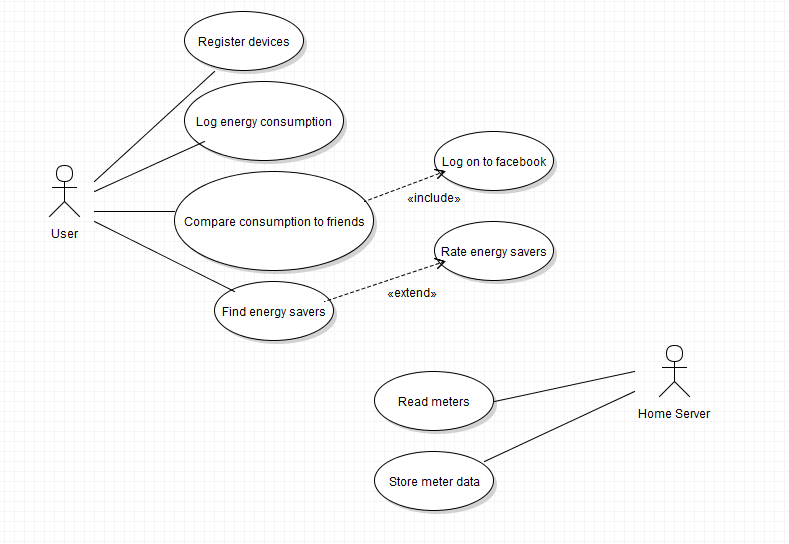
\includegraphics[width=\textwidth]{ch/specification/fig/usecase.png}
\caption{Graphical use case of the entire system.}
\label{fig:usecase}
\end{figure}

Devices

\rowcolors{0}{darkgray}{lightgray}
\begin{table}[H]
\begin{tabular}{|l|p{11.7cm}|}
\hline
\textbf{ID:} 1&\textbf{Overview of devices}\\\hline
\textbf{Actor} &User\\\hline
\textbf{Description}&
The user should be able to see which devices in his house that actually use or produce electricity.\\\hline
\textbf{Preconditions}&
1. Devices are registered\newline
2. Devices are connected to energy measurement device\newline
3. Devices are active\newline
Depends on x.\\\hline
\textbf{Input}&
Registered energy usage\\\hline
\textbf{Post-conditions}& App displays list of all active devices\\\hline
\textbf{Basic flow}&
1. User taps ''Devices''-tab in menu
2. All active devices are displayed in list\\\hline
\textbf{Alternative flow}&
1.1 User taps wrong menu tab. Return to basic flow 1.\\\hline
\end{tabular}
\caption{Textual use case 1}
\end{table}


\rowcolors{0}{darkgray}{lightgray}
\begin{table}[H]
\begin{tabular}{|l|p{11.7cm}|}
\hline
\textbf{ID: }2&\textbf{Display energy usage per device}\\\hline
\textbf{Actor} &User\\\hline
\textbf{Description}&
The user should be able to see how much electricity each device in his house use on a monthly basis and on a yearly basis.\\\hline
\textbf{Preconditions}&
1. Devices are registered\newline
2. Devices are connected to energy measurement device\newline
Depends on x.\\\hline
\textbf{Input}&
Registered energy usage\\\hline
\textbf{Post-conditions}& App displays sector graph where each area represents a device\\\hline
\textbf{Basic flow}&
1. User taps ''Usage''-tab in menu\newline
2. User taps ''Show devices''\newline
3. User wants to display graphs for specific time period\newline
3.a User choose ''Last month'' in drop down menu (default view)\newline
3.b User choose ''Last year'' in drop down menu\\\hline
\textbf{Alternative flow}&
3.1 No electricity usage is registered. Average consumption is displayed.\newline
3.1.a User choose ''Last month'' in drop down menu (default view)\newline
3.1.b User choose ''Last year'' in drop down menu\\\hline
\end{tabular}
\caption{Textual use case 2}
\end{table}

\begin{comment}
\rowcolors{0}{darkgray}{lightgray}
\begin{table}[H]
\begin{tabular}{|l|p{11.7cm}|}
\hline
\textbf{ID:} 3&\textbf{Turn off device}
\\\hline
\textbf{Actor} &User
\\\hline
\textbf{Description}&
User should be able to turn off devices from the app.\\\hline
\textbf{Preconditions}&
1. Device is connected to app.
\newline
2. Device is not a critical device.
\newline
3. The device must be functional.
\newline
4. The device must be turned on.
\newline
Depends on x.\\\hline
\textbf{Input}&
User presses ''Turn off''-button
\\\hline
\textbf{Post-conditions}& 
Device is turned off.
\\\hline
\textbf{Basic flow}&
1. User taps ''Devices''\newline
2. User taps the specific device he wants to turn off\newline
3. User turns off device by pressing ''Turn off''-button
\\\hline
\textbf{Alternative flow}&
2.1 User taps wrong device. Return to basic flow 2.\newline
2.2 User turns off wrong device.\newline
2.2.a User turns on the wrongly selected device. See use case scenario 4.\newline
2.2.b User turns off the correct device. Return to basic flow 3.
\\\hline
\end{tabular}
\caption{Textual use case 3}
\end{table}
\end{comment}

\begin{comment}
\rowcolors{0}{darkgray}{lightgray}
\begin{table}[H]
\begin{tabular}{|l|p{11.7cm}|}
\hline
\textbf{ID: }4&\textbf{Turn on device}
\\\hline
\textbf{Actor} &User
\\\hline
\textbf{Description}&
User should be able to turn on devices from the app.\\\hline
\textbf{Preconditions}&
1. Device is connected to app.\newline
2. The device must be functional. \newline
3. The device must be turned off. \newline
Depends on x.\\\hline
\textbf{Input}&
User presses ''Turn on''-button
\\\hline
\textbf{Post-conditions}& 
Device is turned on.
\\\hline
\textbf{Basic flow}&
1. User taps ''Devices''\newline
2. User taps the specific device he wants to turn on\newline
3. User turns on device by pressing ''Turn on''-button\newline
\\\hline
\textbf{Alternative flow}&
2.1 User taps wrong device. Return to basic flow 2.\newline
2.2 User turns on wrong device.\newline
2.2.a User turns off the wrongly selected device. See use case scenario 3\newline
2.2.b User turns on the correct device. Return to basic flow 3\newline
\\\hline
\end{tabular}
\caption{Textual use case 4}
\end{table}
\end{comment}

\begin{comment}
\rowcolors{0}{darkgray}{lightgray}
\begin{table}[H]
\begin{tabular}{|l|p{11.7cm}|}
\hline
\textbf{ID: }5&\textbf{Specify a maximum of power consumption}
\\\hline
\textbf{Actor} &User
\\\hline
 \textbf{Description}&
The user should have the ability to specify a maximum of power consumption per day for a given device.\\\hline
\textbf{Preconditions}&
1. Device is registered\newline
2. Device is not a critical device\newline
3. Device is connected to app\newline
4. Device is turned on \newline
Depends on x.\\\hline
\textbf{Input}&
User registers maximum kwh/day
\\\hline
\textbf{Post-conditions}& 
Device is turned off when maximum power consumption limit is reached.
\\\hline
\textbf{Basic flow}&
1. User taps ''Devices''-tab in menu\newline
2. User taps specific, correct device\newline
3. User sets maximum power consumption limit
\\\hline
\textbf{Alternative flow}&
2.1 User taps the wrong device. Return to basic flow 2.\newline
3.1 User gives invalid input\newline
3.1.a Error message appears\newline
3.2.a User inputs valid input
\\\hline
\textbf{Comments}& Not available for critical devices\\\hline
\end{tabular}
\caption{Textual use case 5}
\end{table}
\end{comment}

\begin{comment}
\rowcolors{0}{darkgray}{lightgray}
\begin{table}[H]
\begin{tabular}{|l|p{11.7cm}|}
\hline
\textbf{ID: }6&\textbf{Schedule device’s consumption}
\\\hline
\textbf{Actor} &User
\\\hline
\textbf{Description}&
The user should have the ability to schedule when he want a device to consume power. If he want the heat to be off while he is at work, for instance.\\\hline
\textbf{Preconditions}&
1. Device is connected to app\newline
2. Device is registered\newline
3. Device is turned on\newline
4. User has scheduled a specific device\newline
5. Device is not a critical device\newline
Depends on x.\\\hline
\textbf{Input}&
Deviceid, time period
\\\hline
\textbf{Post-conditions}& 
The specific device is turned off in the chosen time period.
\\\hline
\textbf{Basic flow}&
1. User taps ''Devices''-tab in menu\newline
2. User taps specific, correct device\newline
3. User choose a time period
\\\hline
\textbf{Alternative flow}&
2.1 User taps wrong device. Return to basic flow 2.\newline
3.1 User chooses an invalid time period. \newline
3.1.a User receives error message\newline
3.1.b User inputs valid time period.
\\\hline
\textbf{Comments}& Not available for critical devices\\\hline
\end{tabular}
\caption{Textual use case 6}
\end{table}
\end{comment}

\begin{comment}
\rowcolors{0}{darkgray}{lightgray}
\begin{table}[H]
\begin{tabular}{|l|p{11.7cm}|}
\hline
\textbf{ID: }7&\textbf{Notification if the device’s power consumption reaches maximum limit}
\\\hline
\textbf{Actor} &System
\\\hline
\textbf{Description}&
The user should have the ability to specify a maximum of power consumption per day for a given device and the system should notify the user if the device’s power consumption reaches that limit.\\\hline
\textbf{Preconditions}&
1. Device’s maximum limit is specified\newline
2. Device is not a critical device\newline
3. Device is connected to app\newline
4. Device is turned on\newline
5. Device is registered\newline
6. The limit has been reached\newline
Depends on x.\\\hline
\textbf{Input}&
Boolean value that checks whether the usage is higher than the specified maximum kwh/day.
\\\hline
\textbf{Post-conditions}& 
System sends notification to user about the device in question. User receives notification.
\\\hline
\textbf{Basic flow}&
1. System sends notification to user about the device in question. \newline
2. User receives notification.\newline
\\\hline
\textbf{Alternative flow}&\\\hline
\textbf{Comments}& Not available for critical devices\\\hline
\end{tabular}
\caption{Textual use case 7}
\end{table}
\end{comment}


\rowcolors{0}{darkgray}{lightgray}
\begin{table}[H]
\begin{tabular}{|l|p{11.7cm}|}
\hline
\textbf{ID: }8&\textbf{Adding Power Savers}
\\\hline
\textbf{Actor} &User
\\\hline
\textbf{Description}&
The user should be able to add his own Power Savers, steps that have been taken in order to decrease power consumption.\\\hline
\textbf{Preconditions}&
1. User is logged in.\newline
Depends on x.\\\hline
\textbf{Input}&
Description of users Power Saver.
\\\hline
\textbf{Post-conditions}& 
The Power Saver is added to the public database and is visible for other users.
\\\hline
\textbf{Basic flow}&
1. System sends notification to user about the device in question. \newline
2. User receives notification.\newline
\\\hline
\textbf{Alternative flow}&\\\hline
\end{tabular}
\caption{Textual use case 8}
\end{table}


\rowcolors{0}{darkgray}{lightgray}
\begin{table}[H]
\begin{tabular}{|l|p{11.7cm}|}
\hline
\textbf{ID: }9&\textbf{Choosing anonymity}
\\\hline
\textbf{Actor} &User
\\\hline
\textbf{Description}&
The user has a profile connected to his Facebook-account, but he should be able to choose whether the data he aggregates is to be used for comparison against others.\\\hline
\textbf{Preconditions}&
1. User is logged in.\newline
Depends on x.\\\hline
\textbf{Input}&
User's choice.
\\\hline
\textbf{Post-conditions}& 
Anonymity settings based on user's choice.
\\\hline
\textbf{Basic flow}&
1. User taps profile tab.\newline
2. User taps anonymity button.\newline
3. User is prompted with the choice to stay anonymous.\newline
\\\hline
\textbf{Alternative flow}&\\\hline
\end{tabular}
\caption{Textual use case 9}
\end{table}

\begin{comment}
\rowcolors{0}{darkgray}{lightgray}
\begin{table}[H]
\begin{tabular}{|l|p{11.7cm}|}
\hline
\textbf{ID: }10&\textbf{Show a wishlist of items }
\\\hline
\textbf{Actor} &User
\\\hline
\textbf{Description}&
The user should be able to add items with a name and a given price. He should later be able to track his savings up against the values of the items he has entered in the list.\\\hline
\textbf{Preconditions}&
1. User is logged in.\newline
Depends on x.\\\hline
\textbf{Input}&
Name, price, and an url (optional) for an item the user's wishes for
\\\hline
\textbf{Post-conditions}& 
A list of items with their cost, followed by how much of that item the user has saved
\\\hline
\textbf{Basic flow}&
1. The user taps the profile tab
2. The user taps the wish list button
3. The user adds an item with name and cost
4. The user views the list with a progress bar representing his energy savings\newline
\\\hline
\textbf{Alternative flow}&
4.1 The user does not have any consumption data, and therefore no progress is shown on the item
\\\hline
\end{tabular}
\caption{Textual use case 10}
\end{table}
\end{comment}

\begin{comment}
\rowcolors{0}{darkgray}{lightgray}
\begin{table}[H]
\begin{tabular}{|l|p{11.7cm}|}
\hline
\textbf{ID: }11&\textbf{Showing power savings in desired currency}
\\\hline
\textbf{Actor} &User
\\\hline
\textbf{Description}&
The application should project savings in consumption in a currency chosen by the user.\\\hline
\textbf{Preconditions}&
1. User is logged in.\newline
Depends on x.\\\hline
\textbf{Input}&
Desired currency\\\hline
\textbf{Post-conditions}& 
All savings in the application are projected in the chosen currency\\\hline
\textbf{Basic flow}&
1. User taps profile tab\newline
2. User taps currency button\newline
3. User chooses desired currency from lists
\\\hline
\textbf{Alternative flow}&
3.1 User cannot find desired currency in list
\\\hline
\end{tabular}
\caption{Textual use case 11}
\end{table}
\end{comment}

\begin{comment}
\rowcolors{0}{darkgray}{lightgray}
\begin{table}[H]
\begin{tabular}{|l|p{11.7cm}|}
\hline
\textbf{ID: }12&\textbf{Changing the display language of the application.}
\\\hline
\textbf{Actor} &User
\\\hline
\textbf{Description}&
The user should be able to change the language of the application.\\\hline
\textbf{Preconditions}&
1. User is logged in.\newline
Depends on x.\\\hline
\textbf{Input}&
Desired language of operation.\\\hline
\textbf{Post-conditions}& 
The application uses the chosen language.\\\hline
\textbf{Basic flow}&
1. User taps the profile tab\newline
2. User taps the language button\newline
3. User selects desired language from list
\\\hline
\textbf{Alternative flow}&
3.1 User cannot find desired language in list
\\\hline
\textbf{Comments}&Only a limited amount of languages will be available upon release. \\\hline
\end{tabular}
\caption{Textual use case 12}
\end{table}
\end{comment}

\rowcolors{0}{darkgray}{lightgray}
\begin{table}[H]
\begin{tabular}{|l|p{11.7cm}|}
\hline
\textbf{ID: }13&\textbf{Sharing power savings on Facebook}
\\\hline
\textbf{Actor} &User
\\\hline
\textbf{Description}&
The user should be able to share any savings in monthly consumption with his friends on Facebook.\\\hline
\textbf{Preconditions}&
1. User is logged in with Wattitude on Facebook\newline
Depends on x.\\\hline
\textbf{Input}&
Users credentials for Facebook account.\\\hline
\textbf{Post-conditions}& 
The data is shared on Facebook. \\\hline
\textbf{Basic flow}&
1. OBSOBS, endre her? The user taps the social tab\newline
2. The user taps share\newline
3. The user selected the data he wants to share, and what accounts to share it on\newline
4. Preformatted messages with the given data is posted to the social media accounts
\\\hline
\textbf{Alternative flow}&
4.1. The social accounts do not allow the application to post
\\\hline
\end{tabular}
\caption{Textual use case 13}
\end{table}

\rowcolors{0}{darkgray}{lightgray}
\begin{table}[H]
\begin{tabular}{|l|p{11.7cm}|}
\hline
\textbf{ID: }14&\textbf{Connecting with friends whom are using the application}
\\\hline
\textbf{Actor} &User
\\\hline
\textbf{Description}&
The user should be able to find and connect to his friends through Facebook.\\\hline
\textbf{Preconditions}&
1. User is logged in.\newline
Depends on x.\\\hline
\textbf{Input}&
User's Facebook credentials.\\\hline
\textbf{Post-conditions}& 
A list of friends currently using the application.\\hline
\textbf{Basic flow}&
1. The user taps the social tab
\\\hline
\textbf{Alternative flow}&
1.1. The user does not have any friends currently using the application
\\\hline
\end{tabular}
\caption{Textual use case 14}
\end{table}


\rowcolors{0}{darkgray}{lightgray}
\begin{table}[H]
\begin{tabular}{|l|p{11.7cm}|}
\hline
\textbf{ID: }15&\textbf{Comparison of data and power savers}
\\\hline
\textbf{Actor} &User
\\\hline
\textbf{Description}&
The user should be able to compare his power usage and power savers with friends or other people in the area\\\hline
\textbf{Preconditions}&
1. User is logged in\newline
2. User has logged energy consumption data\newline
Depends on x.\\\hline
\textbf{Input}&
The users energy consumption data or power savers.\\\hline
\textbf{Post-conditions}& 
Application displays a list of friends and their respective energy consumption. A list of energy savers implemented by friends is also available. \\\hline
\textbf{Basic flow}&
1. The user taps the social tab\newline
2. The user taps the compare button\newline
3. The system retrieves the users friends and graphs their consumption against his own logged consumption\newline
4. Power savers from friends and others is also available
\\\hline
\textbf{Alternative flow}&
3.1. The does not have any friends currently using the application
\\\hline
\end{tabular}
\caption{Textual use case 15}
\end{table}